\section{Motivation}
\label{sec:motivation}

\subsection{Ordering Anomalies}
\label{subsec:tso}

In a traditional distributed system where the network is unreliable and has arbitrary delay, several categories of ordering anomalies may take place.

\textbf{Send after write (SAW)}. As shown in Figure~\ref{fig:causality_traditional}, $A$ writes data to a remote shared storage $O$ and sends a message to notify $B$. Then $B$ reads $O$, but may get nothing.

\textbf{Write after write (WAW)}. $A$ writes data to shared storage $O$, then writes metadata to shared storage $X$. Asynchronously, $B$ reads $X$ and gets the metadata, then attempts to fetch data from $O$, but may get nothing.

\textbf{Independent multi-write (IMW)}. $S_1$ and $S_2$ are two web servers, generating an access log to $A$ and an error log to $E$ for each HTTP request. The interleaving order of requests from $S_1$ and $S_2$ may be different at $A$ and $E$.

\textbf{Independent read, independent write (IRIW)}. Client $R$ reads two remote shards while another client $W$ writes the two shards. $R$ may get an inconsistent state where only one of the shards is written by $W$.


In today's distributed systems, to avoid RAW and WAW hazards, $A$ needs to wait for the first write operation to complete (an RTT to the shared storage) until issuing the next operation, therefore increases latency and limits concurrency. To avoid IMW and IRIW hazards, application needs locks or explicit coordination via logical timestamps~\cite{lamport1978time}.

These ordering anomalies have been studied extensively in shared memory systems. Recent processors provide higher memory consistency models. In particular, x86 ensures a \textit{total store ordering} (TSO) memory model~\cite{sewell2010x86} where each core observes a consistent ordering of writes from all other cores. In other words, remote writes are propagated via total order communication. TSO eliminates SAW and WAW ordering anomalies above, making multi-core concurrent programming much easier to reason. In addition, TSO makes \textit{memory barrier} easy to implement without locking the bus. The barrier initiator core blocks itself and sends a message to itself via total order communication, and unblocks upon receiving the message. In this paper, we extend the concept of TSO to distributed systems, providing same consistency as multi-core processors. In Sec.\ref{subsec:transactional-kvs}, we introduce a message scattering primitive to remove IMW and IRIW hazards. %Concretely, each message is assigned a monotonically increasing timestamp at the sender and each receiver processes messages in timestamp order (break ties by sender ID).

\iffalse
\begin{figure}[t]
\centering
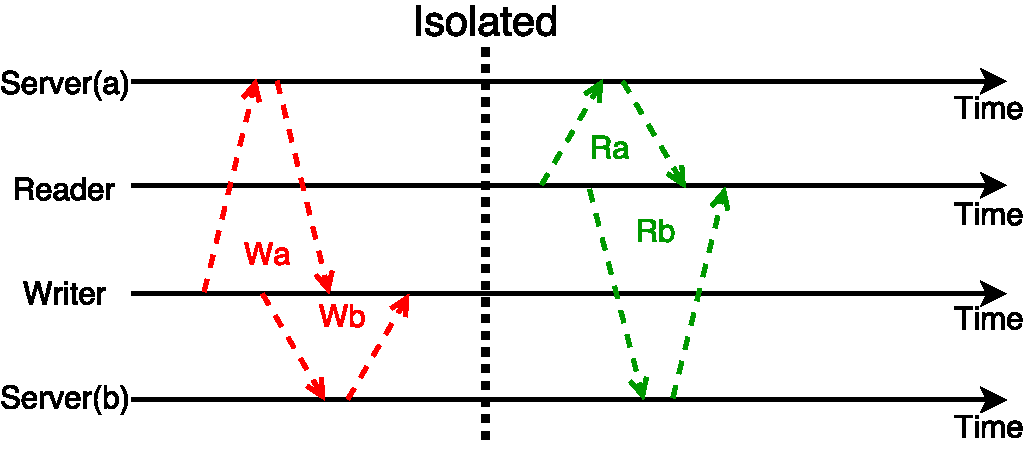
\includegraphics[width=0.48\textwidth]{images/read_write_isolation.pdf}
\caption{Two senders issue read and write requests to two receivers.}
\label{fig:example}
\end{figure}



\begin{figure}[t]
\centering
	\subfloat[Lock-based.\label{fig:concurrency-lock}]
	{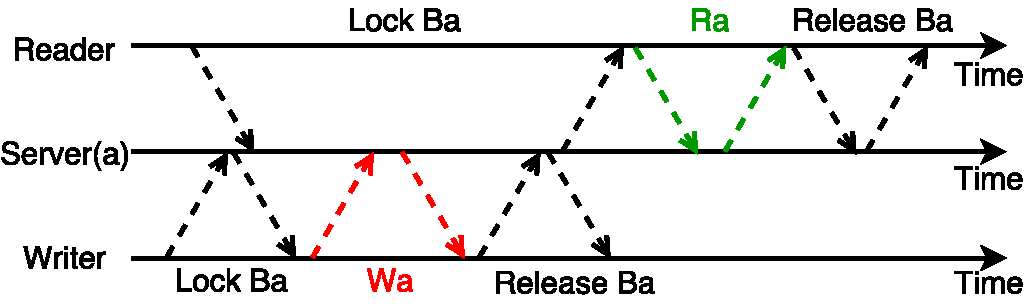
\includegraphics[width=.45\textwidth]{images/LockBased.pdf}}
    \hspace{0in}
	\subfloat[Timestamp-based (OCC).\label{fig:concurrency-timestamp}]
	{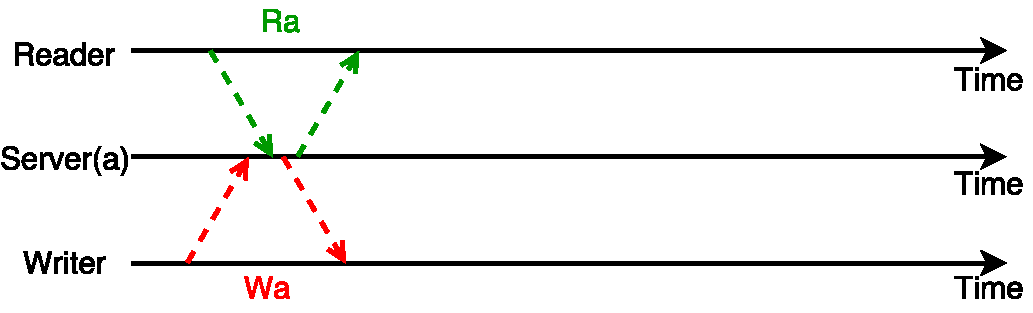
\includegraphics[width=.45\textwidth]{images/TimestampBased.pdf}}
	\caption{Two concurrency control mechanisms for distributed transactions.}
	\label{fig:concurrency-control}
\end{figure}
\fi


\begin{figure}[t]
\centering
	\subfloat[Possible causality violation due to variable network delay.\label{fig:causality_traditional}]
	{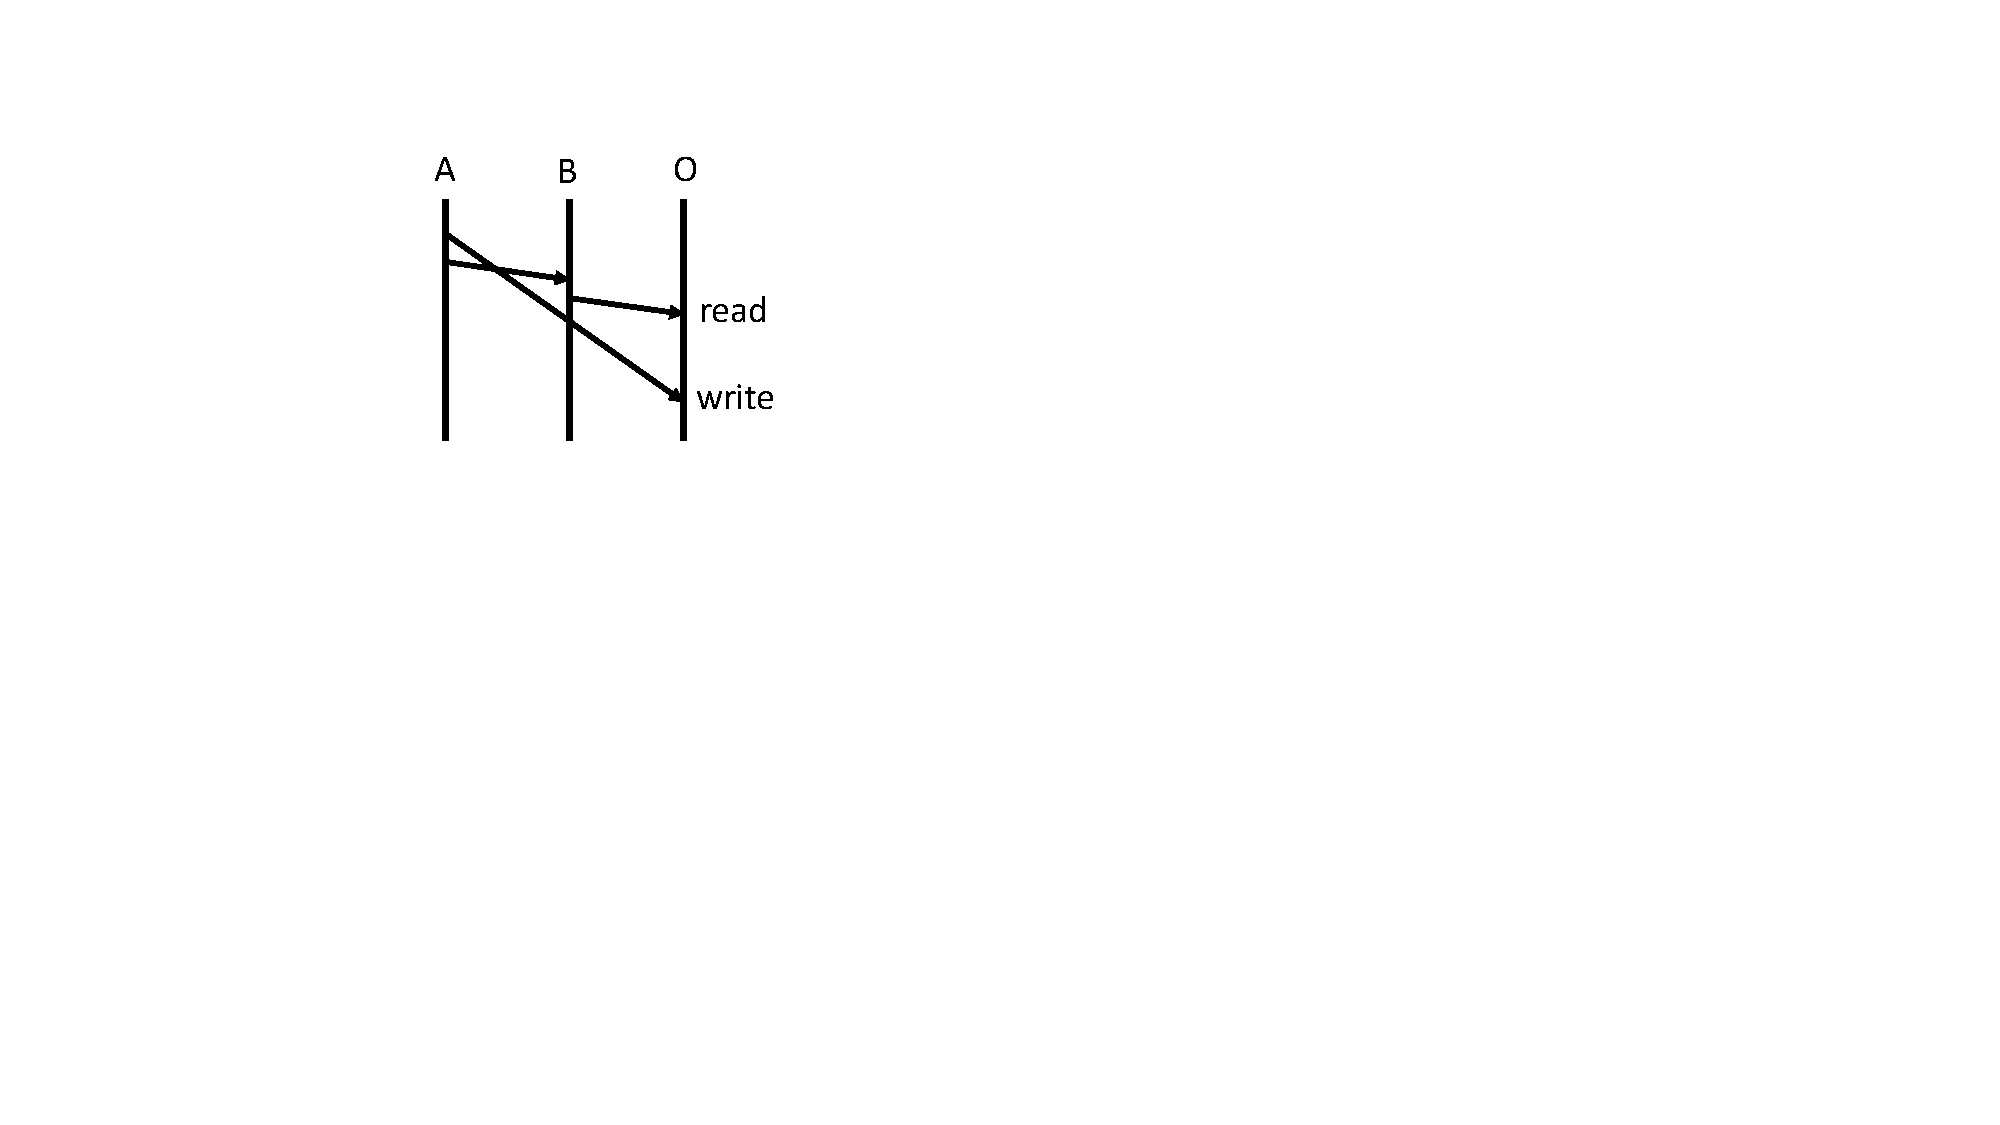
\includegraphics[width=.2\textwidth,page=1]{images/cropped_causality.pdf}}
    \hspace{0.03\textwidth}
	\subfloat[Guaranteed causality in \sys.]
	{\includegraphics[width=.2\textwidth,page=2]{images/cropped_causality.pdf}}
	\caption{Causality example: $A$ write shared object $O$, then notify $B$, then $B$ read $O$.}
	\label{fig:causality}
	\vspace{-1.5em}
\end{figure}


%The story begins with a hypothetical distributed banking system. Two accounts Alice and Bob are stored in different \textit{shards} at distant locations. Initially, their balances are $B_a$ and $B_b$. When Alice transfers \$1 to Bob, two write operations are sent to the shards: $B_a -= 1$ and $B_b += 1$, call them $W_a$ and $W_b$. At the same time, an auditor checks the total balance in the bank by accumulating balances of all accounts, resulting in two read operations: $R_a$ and $R_b$.
%If the system does not support transactions, the ordering of events may be $W_a < R_a < R_b < W_b$, then the auditor would find an inconsistent total balance.

%It is worth noting that \sys ensures ordering instead of consensus. When some hosts experience failure, \sys does not ensure a quorum of hosts agree on its received messages. NOPaxos~\cite{li2016just} has shown that \sys leads to an efficient implementation of distributed consensus.


\subsection{Serializable Log Replication}
\label{subsec:log-replication}

A ubiquitous application of total order communication is \textit{log serialization}. Distributed databases are replicated for reliability and performance. When multiple replicas process write operations in parallel, the consistency among replicas is a paramount challenge. The PACELC theorem~\cite{abadi2012consistency} suggests that even when a system has no failure and network partition, one has to choose between latency (L) and consistency (C). On one end of the spectrum are strongly consistent systems, where each replica processes read operations locally and requires an RTT for write operations to propagate to all replicas. Low latency data center networks enable an increasing number of intra-datacenter databases embrace strong consistency. On the other end of spectrum are eventually consistent systems, where both read and write operations can be processed locally, and conflicting write operations are merged in a deterministic way. Due to high latency among data centers, most geographically replicated databases choose eventual consistency.

Total order communication ensures that each replica receives an identical sequence of write operations from other replicas. If write operations are blocked until receiving potentially conflicting writes, \textit{i.e.} insert a memory barrier after each write, the system is sequentially consistent because each operation can be serialized at its beginning time. If write operations are returned immediately while changes propagate, because local read operations may occur during propagation, the system is not sequentially consistent, but causality and eventual consistency are preserved. Applying the last-writer-wins rule \RED{cite} on the timestamps of local objects and remote updates achieves eventual consistency. The reasoning above assumes reads are local and writes are propagated. Similar reasoning applies to write-intensive systems where writes are local, while each read operation retrieves from multiple replicas and return the latest version. Total order communication also ensures sequential consistency in this case.

The predominant approach to total order communication is consensus protocols~\cite{lamport1998part,raft}, which introduces a centralized serialization point (not necessarily on the data path, but at least requires a centralized sequencer~\cite{kaminsky2016design}). Due to scalability concerns of log serialization~\cite{anna}, there has been extensive work to track operation dependency and ensure convergent conflict resolution at application level (COPS, Eiger, RedBlue...). First, most of these approaches do not address IRIW hazard. Second, they cannot say ``for sure'' in the presence of out-of-band communication~\cite{cheriton1994understanding}, \textit{e.g.} cannot avoid SAW hazard if send operation is not tracked in the dependency graph. In addition to higher consistency, total order communication provides an explicit time of convergence. After receiving replication of timestamp $T$, we are sure that the history before $T$ will never be changed.

\subsection{Atomic Multi-Shard Operations}
\label{subsec:transactional-kvs}

Memory consistency and log replication motivate the need of total order multicast, where one message is sent to multiple receivers. In addition, applications need serializable execution of a group of operations~\cite{cheriton1994understanding}, \textit{e.g.} accessing metadata and data. If a group of operations involve multiple shards in a distributed system, the communication pattern is \textit{message scattering}, where one sender scatters potentially different messages to multiple receivers. The messages in a scattering should be ordered \textit{atomically}, such that a) either all or none receivers deliver the messages, b) all messages are delivered at a same serialization time. The IMW and IRIW cases in Sec.\ref{subsec:tso} are examples of message scattering. In IMW, access and error log of a request compose a scattering. In IRIW, two read requests and two write requests each compose a scattering.

Atomic message scattering is equivalent to the concurrency control problem in single round-trip transactions (or called one-shot transactions). There are two main categories of concurrency control. One category uses \textit{locks} to protect accesses to shared resources. In this way, the transaction throughput is bounded by the RTT between the clients and the shards. The other category is \textit{optimistic concurrency control} (OCC), which assigns a \textit{timestamp} to each transaction (or scattering). Transactions are serialized according to timestamp order. Due to variable network delay, shards may receive transactions out-of-order. Out-of-order transactions are aborted and retried with a higher timestamp. The abort rate increases with the number of concurrent conflicting transactions. \sys transfers a single round-trip transaction as a message scattering, which ensures that shards process transactions in timestamp order, therefore eliminating transaction aborts. In the absence of packet loss and node failure, atomic multi-shard operations can complete in an RTT, adding little latency and bandwidth overhead compared to non-atomic operations.

%We will use a hypothetical banking example to illustrate the main concepts. Two accounts Alice and Bob are stored in different \textit{shards} at distant locations. Initially, their balances are $B_a$ and $B_b$. When Alice transfers \$1 to Bob, two write operations are sent to the shards: $B_a -= 1$ and $B_b += 1$, call them $W_a$ and $W_b$. At the same time, an auditor checks the total balance in the bank by accumulating balances of all accounts, resulting in two read operations: $R_a$ and $R_b$. If the system does not support transactions, the ordering of events may be $W_a < R_a < R_b < W_b$, then the auditor would find an inconsistent total balance.

%A strongly consistent distributed system requires the reads and writes to be \textit{transactional}. The transaction $R_a, R_b$ and the transaction $W_a, W_b$ need to be performed in isolation.

%There are two main categories of concurrency control to implement a transactional system. One category uses \textit{locks} to protect accesses to shared resources. The read transaction needs to lock $B_a$ and $B_b$, and the write transaction also needs to lock them. The transaction throughput is bounded by the \textit{round-trip time} (RTT) between the clients and the shards, because the lock must be sent from the shard to the client, then the client may send unlock to the shard.
%In our example scenario where all transactions need to lock a single resource, if the RTT is 100~$\mu$s, the throughput is bounded to 10K transactions per second.

%The other category is \textit{optimistic concurrency control} (OCC). It assigns a \textit{timestamp} to each transaction ($T_R$ for read, $T_W$ for write) and tracks object accesses during transaction execution. Transactions are serialized according to timestamp order. Once the system detects a \textit{late write}, that is, the write operation has lower timestamp than a read operation ($T_W < T_R$) but arrives later ($R_a < W_a$ or $R_b < W_b$), one of the transactions needs to be aborted and retried with a higher timestamp.
%Due to variable delays between clients and shards, if the read and write transactions are initiated at almost the same time, there are many possible orderings of $R_a, R_b, W_a, W_b$ and $T_R, T_W$. 
%If the network delays between clients and shards follow a normal distribution, for two conflicting concurrent transactions, the probability of aborting one transaction is 3/4 with two shards. If each transaction involves $N$ shards, the abort probability is $1-(\frac{1}{2})^N$.

%If we regard each transaction as an event on a client, then the \textit{event timestamp} is the transaction timestamp. The read and write operations are the effects of the events, which propagate to the shards via messages.
%Each event may \textit{scatter} a set of messages to receivers (shards in our example). Each message is tagged with the event timestamp. Different messages may be scattered to different receivers, so \textit{broadcast} is a special case of \textit{scatter}.

%To implement OCC without transaction aborts, we propose \textit{total-order message scattering} (\sys). \sys assigns timestamps to events and scatters messages from events, so that each host delivers messages to applications in monotonically increasing timestamp order (break ties by sender ID).
%\sys provides a total ordering of all events in a distributed system, and ensures that each node observes the events (via messages) consistent with the total ordering.
%With \sys, we regard each single-round-trip transaction as an event on the transaction initiator. In the absence of failure, transaction abort in OCC will never be triggered, because the read and write operations are always received by shards in the same ordering according to transaction timestamps.


%In the distributed system, multiple \textit{hosts} are connected via the network. %A distributed system is made up of multiple \textit{hosts} connected via network. 
%An \textit{event} occurs on a host, and scatters messages to other hosts. For example, a distributed single-round-trip transaction can be regarded as an event on the transaction initiator, and its read and write operations are sent to the shards where the objects are stored. Here we use the term \textit{scatter} instead of \textit{multicast} because each shard only needs to receive operations related to the objects it host.


%Recent years there is rich literature on improving eventual consistency in geographically replicated systems . The CAP theorem suggests that sequential consistency is not possible if both read and write operations have latency lower than inter-datacenter delay.

%COPS and Eiger provide causal+ consistency in geo-replicated systems by tracking dependency of values or operations at shared storage servers. Causal consistency rules out WAW hazard. To rule out SAW hazard, message passing needs to be taken into account when tracking potential causal dependencies. Although causal+ ensures per-key sequential consistency by serializing the update log of each key, in the IRIW case, the change order observed by C and D may eventually diverge, because A and B are different keys. Furthermore, eventually consistent systems typically do not provide a bounded delay of convergence.

%We build each replica as a transactional key-value store, and deploy another instance of reliable TOMS for replication traffic. TOMS serializes updates from all remote replicas. Applying the last-writer-wins rule on the timestamps of local objects and remote updates, the system will be eventually consistent, without the need of tracking causal dependencies or a convergent conflict handling function. TOMS also provides bounded convergence delay. After receiving replication at timestamp T and resolving conflicts, we are sure that the history before T will never be changed. Furthermore, we no longer need to replicate to all replicas to ensure total ordering of updates (cite The Potential Dangers of Causal Consistency and an Explicit Solution, SOCC'12).
